In diesem Unterkapitel wird der Targetdatensatz deutlich verkleinert und hat dann nur noch 240 Datensamples. Es werden dieselben Tests wie 
im vorherigen Unterkapitel durchgeführt. 

% Es wird zuerst angefangen mit Deep Cascade, da es Unterschiede zwischen den beiden Kaskadenversionen gibt. 
% Bei wenigen Targetdaten gibt es einen Unterschied zwischen Deep Cascade und Direct Cascade. Beides läuft zwar etwas schlechter als mit vielen 
% Daten ist aber mit TF unter Umständen besser als ohne. Dabei ist Deep Cascade etwas besser als Direct Cascade. 

\begin{figure}[htpb]
    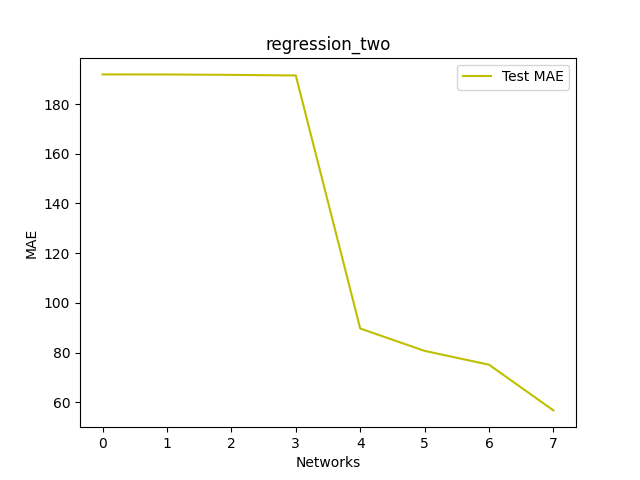
\includegraphics[height=5cm]{../../Plots/ba_plots/regression_small/regr2_ts.png}
    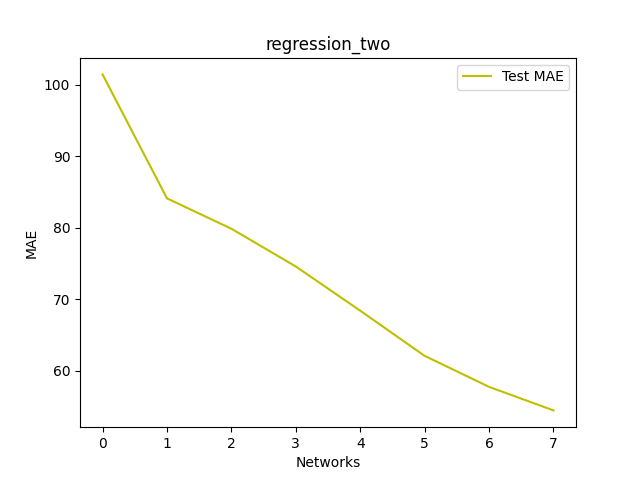
\includegraphics[height=5cm]{../../Plots/ba_plots/regression_small/woregr2_ts.png}
    \caption{\label{fig:smallregr} 
    \small{Hier ist der Vergleich zwischen mit TF und ohne mit wenig Targetdaten auf dem Regr2-Netzwerk zu sehen. 
    Die Tests sind: links Regr2:TF4/240/10/8 und rechts Regr2:240/10/8. Dabei ist zu sehen, dass dieses Netzwerk ohne TF besser läuft als mit.}}
\end{figure}


In Figure 5.4 sind die Ergebnisse des Deep Cascade Netzwerks. Es ist ohne TF tatsächlich besser als mit. Dies liegt daran, dass die Gewichte der 
ersten Hälfte des Netzes nur auf dem Sourcedatensatz passend gelernt haben. 

Es gibt aber deutliche Unterschiede zu Direct Cascade, weshalb beide Netze hier gezeigt werden. 

\begin{figure}[htpb]
    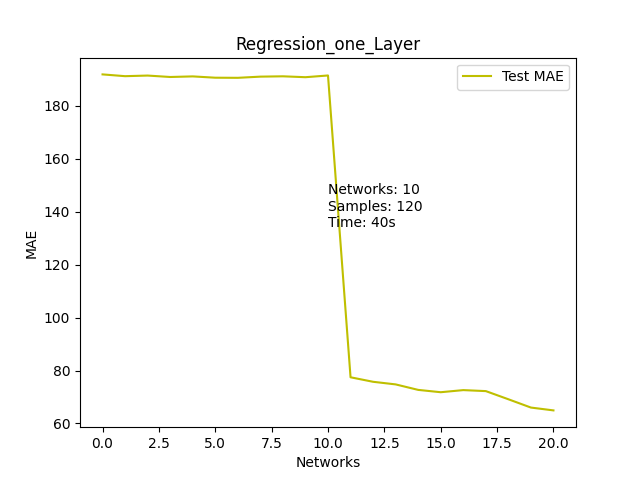
\includegraphics[height=5cm]{../../Plots/ba_plots/regression_small/onelayer_ts.png}
    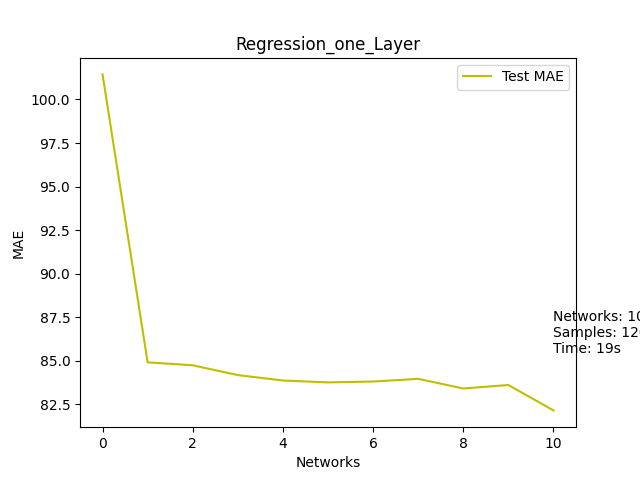
\includegraphics[height=5cm]{../../Plots/ba_plots/regression_small/woonelayer_ts.png}
    \caption{\label{fig:smallonl} 
    \small{Dies ist der Vergleich im 1Lay-Netzwerk im Fall der wenigen Targetdaten zwischen TF und ohne. Die dahinter liegenden Tests sind: 
    links 1Lay:TF11/240/10/21 und rechts 1Lay:240/10/11. Dabei auffällig ist, dass dieses Netzwekr mit TF besser ist als ohne.}}
\end{figure}

Figure 5.5 bezieht sich auf das Direct Cascade Netzwerk. Es wird deutlich, dass in dieser Kaskadierungsvariante das Netz deutlich schlechter 
ohne TF ist als mit. Daran wird erkannt, dass hier positive TF vorliegt. Die Predictions, die mithilfe des Sourcedatensatzes über die 
zu dem Zeitpunkt nicht betrachteten Targetdaten, verbessern das Gesamtergebnis deutlich. Dadurch gibt es mehr Daten pro Sample, wenn auf dem 
Targetdatensatz das Training begonnen wird. Diese Daten sind dabei nicht störend für die Performanz, weshalb es dann besser mit TF ist als ohne. 

Allerdings ist das Deep Cascade Netzwerk sowohl mit als auch ohne TF minimal besser. Dies kann aber auch 
an dem dahinter liegenden Netz liegen, da sie nicht nur die exakt gleichen Layer haben. 
Noch besser ist die Variante, 
die weder Kaskadierung noch TF nutzt, sondern ein komplettes Netzwerk ist, wie in Figure 5.6 gezeigt. 

\begin{figure}
    \centering
    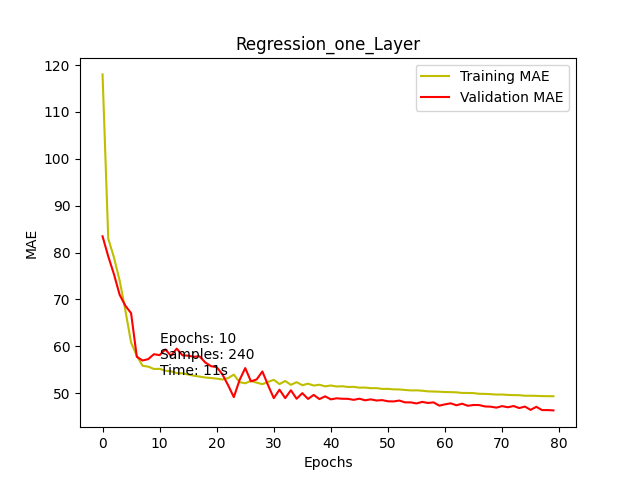
\includegraphics[height=5cm]{../../Plots/ba_plots/regression_small/onelayer_complete.png}
    \caption{\label{fig:smallonlcomp} 
    \small{Hinter diesem Plot ist der Test 1Lay:Comp/240//8. Dieser ist trotz der wenigen Daten erfolgreicher 
    als alle anderen Tests, obwohl dieser weder Kaskadierung noch TF besitzt.}}
\end{figure}

Der MAE-Wert der Testdaten beläuft sich hier auf 53 Tausend Dollar, wäh-rend dieser sonst bei so wenig Datensamples bei 60 bis 80 liegt. 

Also ist ein Netz gänzlich ohne Kaskadierung, aber mit vielen Hidden Layern und nur einem Trainingsaufruf bei 80 Epochen, auch bei wenigen 
Daten besser als diejenigen mit Kaskadierung und kommt sogar an den Wert heran, der mit vielen Daten erreicht wird. 
Dieses Netz hat im Gegensatz zu den Anderen die Möglichkeit zwischen den Layern zu lernen und mit den noch nicht fertig verarbeiteten Daten 
des Inputs weiterzurechnen. Das dürfte dazu beitragen, dass es eine bessere Performanz gibt. 

Wenn diese Tests mit einem explizit großen Testdatensubset angewendet werden, dann ändert sich nur der tatsächliche MAE-Wert dahingehend, dass 
dieser etwas schlechter wird. Die Verhältnisse zwischen den Netzen hingegen nicht. 
